\chapter{\texorpdfstring{\emph{Introduction}}{Introduction}}\label{c1_introduction}

As planetary boundaries are progressively transgressed ---in particular the climate and biosphere-integrity frontiers--- Space Earth Observation Sensors are evolving to match the pace of environmental change and are becoming essential for both mitigation and adaptation.
This thesis contributes to that emerging capability through the mission design of a small-satellite constellation for fire detection, targeting sub-30-minutes revisit and metre-scale ground resolution over continental Portugal with coverage extending to global fire-prone regions, and positions the system within the \emph{Planetary Boundaries} framework (Fig.~\ref{fig:intro_planetary_boundaries}) as a sensor providing a fire-information link, $\mathcal{L}_{\text{fire}}$, connecting the spacecrafts to two ground domains ---fire-stressed ecosystems and human wildfire combat response--- shortening the feedback loop from environmental change to operational action \cite{rockstrom2009safe, richardson2023earth,sakschewski_planetary_2025,lenton_gaia_2018}.


\begin{figure}[H]
    \centering
    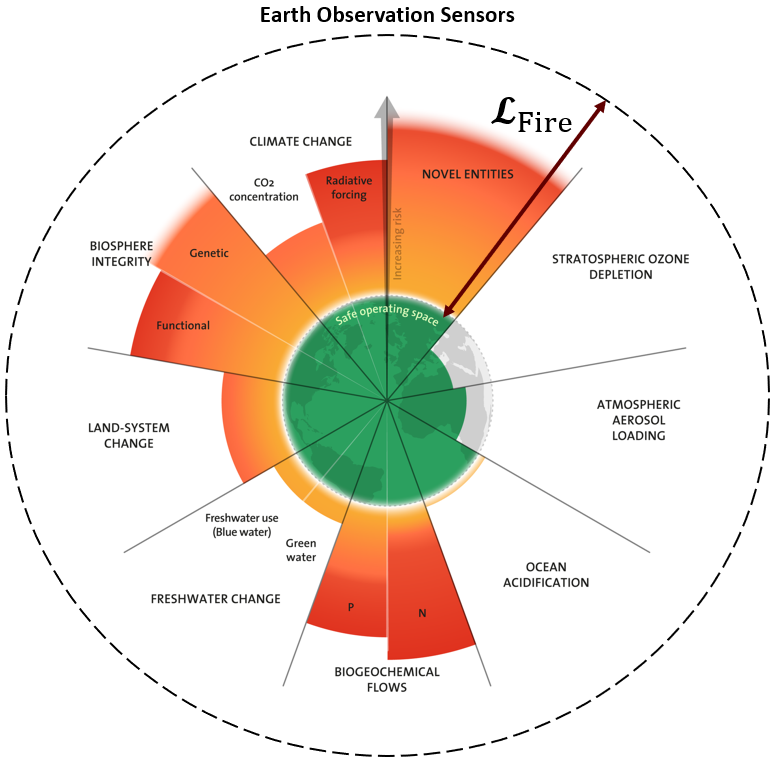
\includegraphics[width=0.65\linewidth]{images/planetary_bondaries_2025_9frontires_7_crossed_Lfire.png}
    \caption{\footnotesize{Planetary boundaries showing the safe operational limit of the Earth system, with the climate boundary transgressed and the biosphere integrity boundary under high risk. \cite{sakschewski_planetary_2025}}}
    \label{fig:intro_planetary_boundaries}
\end{figure}


% \begin{figure}
%     \centering
%     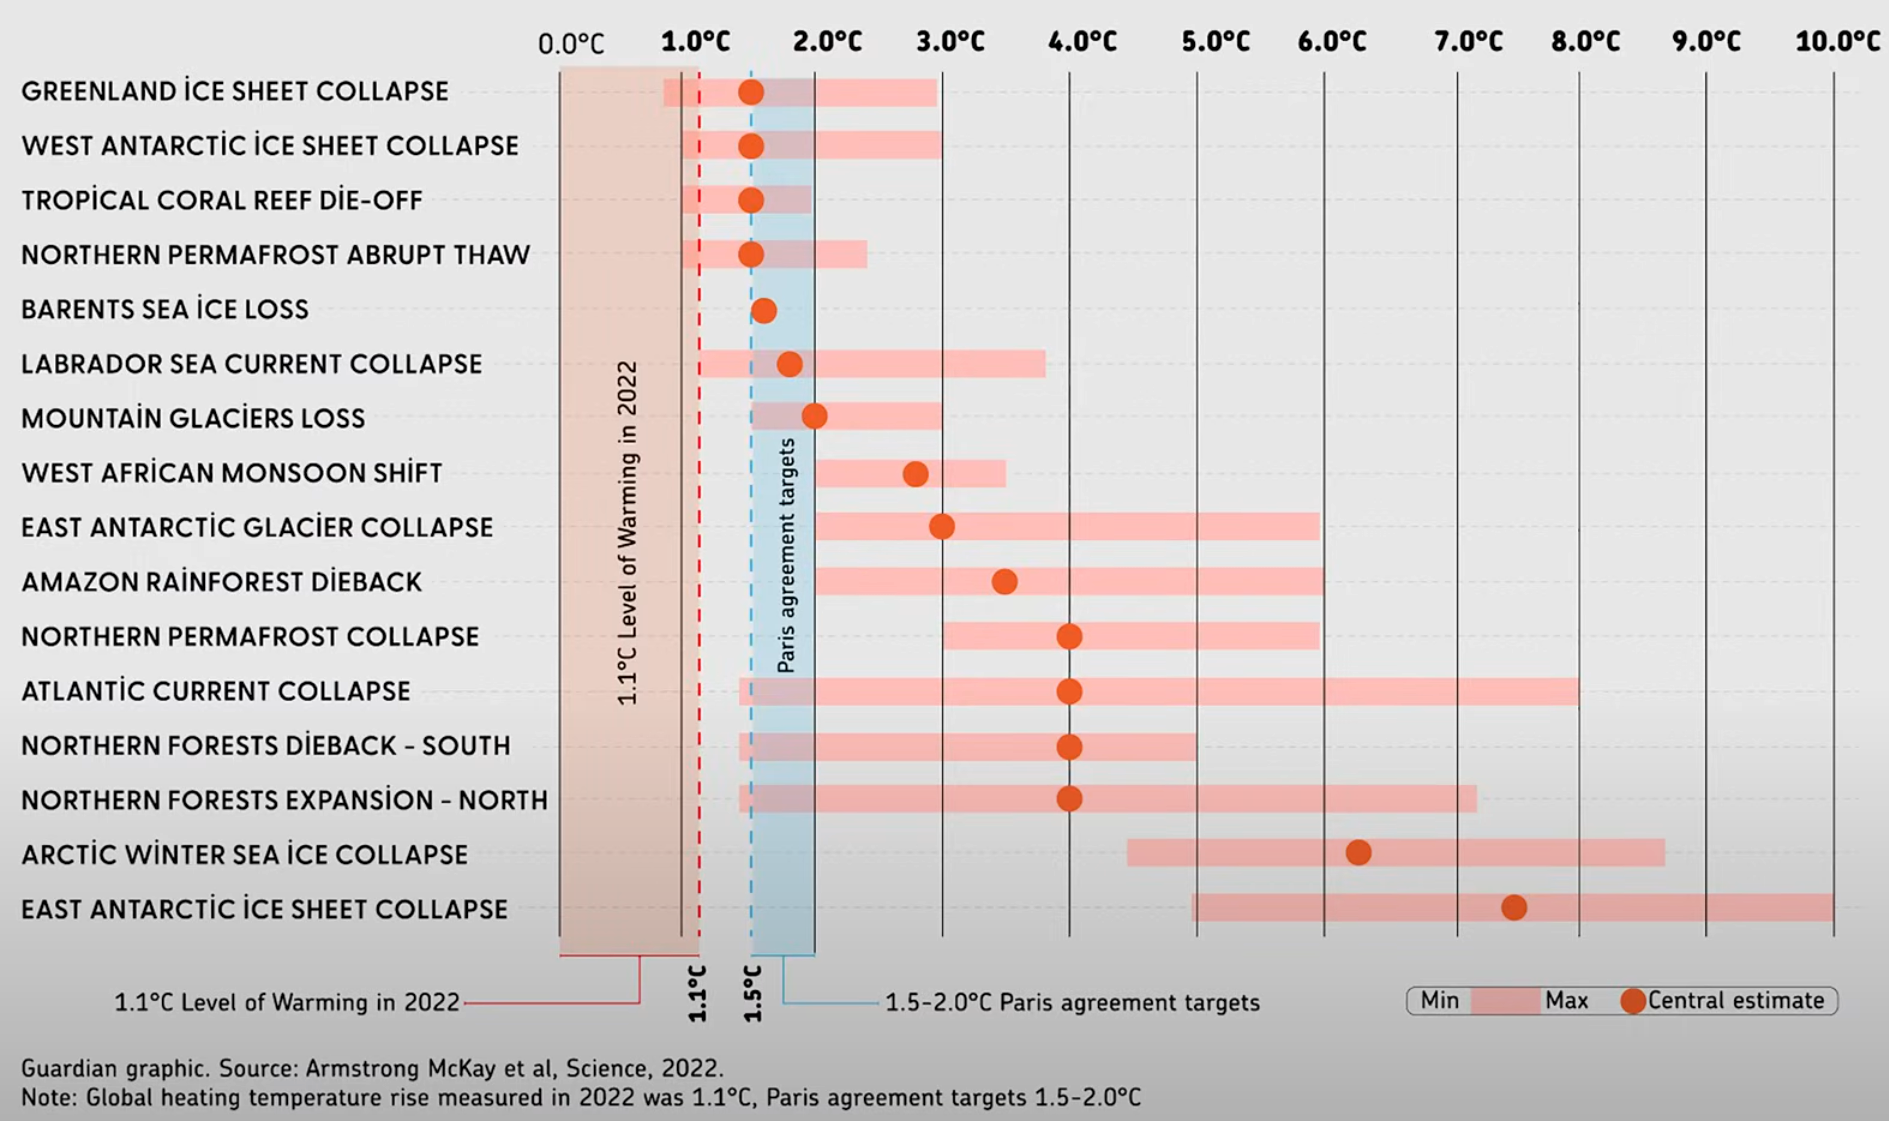
\includegraphics[width=1\linewidth]{images/tiping_points_info.png}
%     \caption{Enter Caption}
%     \label{fig:intro_tipping_points}
% \end{figure}

This thesis mission is also situated within the scope of \emph{Intergovernmental Panel on Climate Change (IPCC) AR6}, as a \emph{cross-sectoral transition system} (items C.2.11, C.2.12, and C.2.13)---an \emph{adaptive response} toward \emph{sustainable and resilient states} in \emph{urban infrastructures}, \emph{terrestrial and coastal 	ecosystems}, and in \emph{social choices/transitions}, providing  \emph{Disaster Risk Management} and \emph{Early Warning Systems}. 
\cite{ipcc2018sr15,ipcc2022wg2,ipcc2023syr}.


\emph{Why acting now is urgent?} In light of the \emph{Paris
	Agreement (Art. 2, UNFCCC)} and \emph{IPCC SR1.5}, limiting warming to
\emph{1.5 °C} requires \emph{net-zero CO\textsubscript{2} around 2050} \cite{ipcc2018sr15,unfccc2015paris}.
The \emph{Glasgow Climate Pact (COP26)} and the
\emph{UNFCCC Global Stocktake} indicate that current progress is
\emph{off-track} \cite{unfccc2021glasgow,unfccc2023gst}, while the \emph{World
	Meteorological Organization (WMO)} reports annual global means near the
\emph{1.5 °C} level in \emph{2023--2024} (temporary exceedances)
\cite{wmo2024state,wmo2025press}. Within \emph{Planetary Boundaries}, the
\emph{climate boundary} is \emph{transgressed}, raising the risk of
cascading impacts; warming around \emph{1.5 °C} increases the
likelihood of \emph{losses of resilience} and \emph{abrupt changes}
\cite{richardson2023earth,lenton2019tipping,armstrong2022tipping}.

% \begin{figure}[H]
%     \centering
%     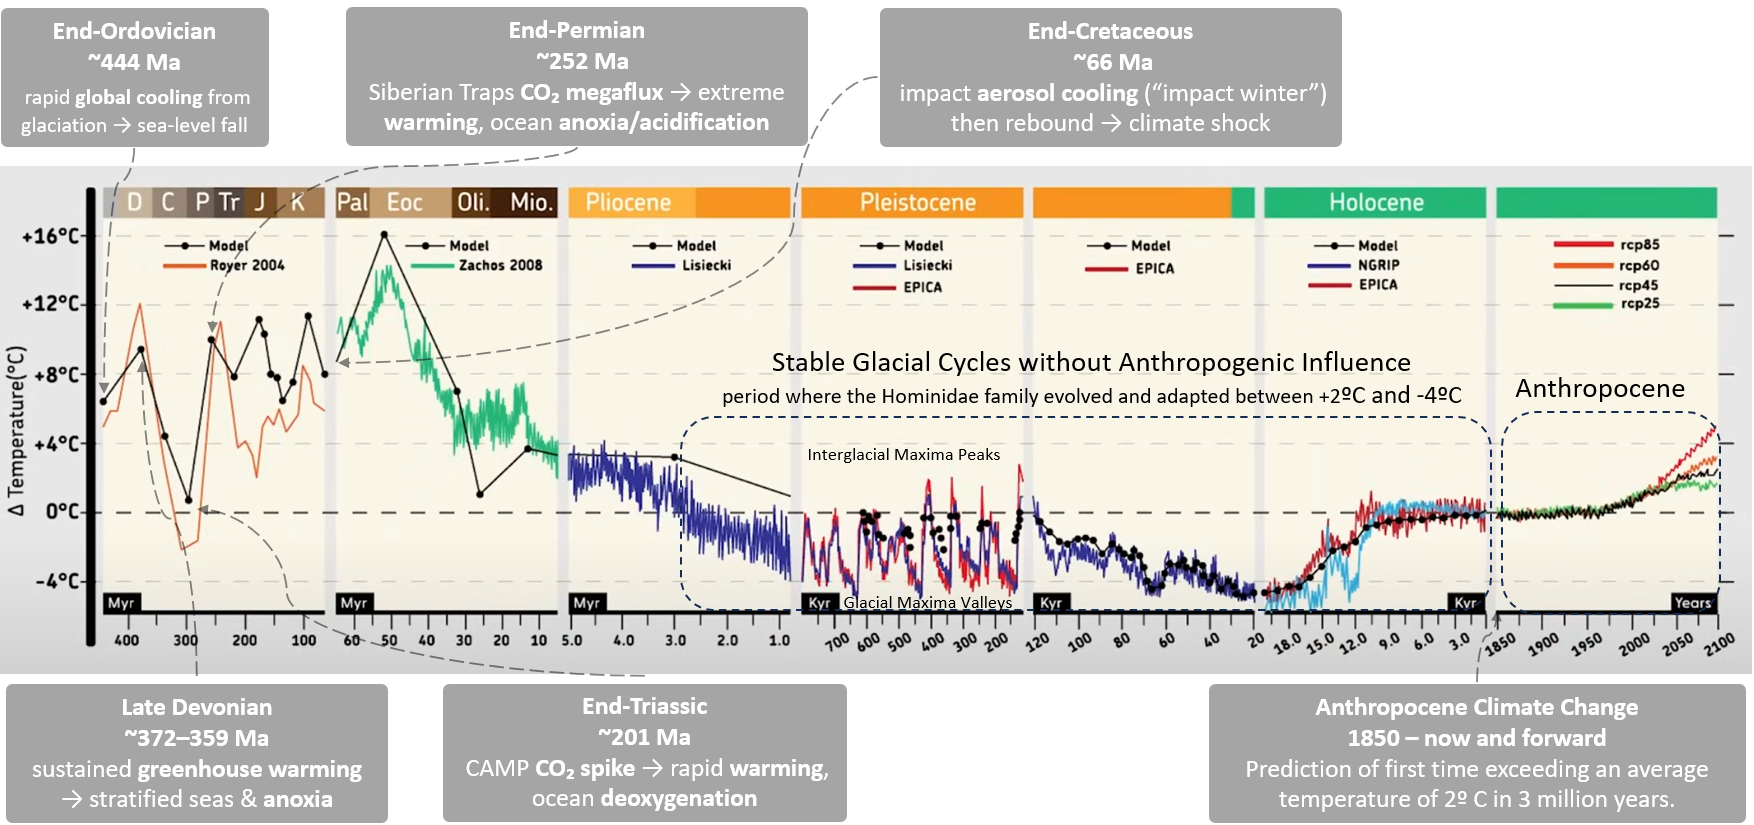
\includegraphics[width=1\linewidth]{images/paleclima_Dt_mass_extitions.png}
%     \caption{\footnotesize{Paleo-weather temperature variation, mass extinctions, and the Anthropocene fire signal.
% Global mean temperature anomalies from multiple compilations show large coincident with the \textbf{Big Five mass extinction}s:  \textbf{I)End-Ordovician (~444 Ma)} : abrupt cooling and glaciation; \textbf{II)Late Devonian (~372–359 Ma)}: greenhouse warming pulses superimposed on a long cooling trend, driving ocean stratification/anoxia; \textbf{III)End-Permian (~252 Ma)}: CO$_2$ megaflux and extreme warming leading to widespread anoxia/acidification; \textbf{IV)End-Triassic (~201 Ma)} rapid volcanogenic warming with ocean deoxygenation; \textbf{V)End-Cretaceous (~66 Ma)}: impact winter (short cooling) followed by rebound warming. The Pleistocene section exhibits \textit{quasi-periodic glacial–interglacial cycles} (early 41 kyr, late ~100 kyr “sawtooth”) within which hominins evolved. During the Holocene, a period with stable temperatures that coincides with and facilitates the development of agriculture and the flourishing of larger human societies. During this epoch, we find the \textbf{Anthropocene, which has as one of its marks an unprecedented, human-driven warming rate}, with high-emission pathways possibly exceeding +2 °C, warmer than any time in ~3 Myr and aligned with multiple planetary-boundary transgressions. In this work, we interpret the documented increase in active fire as an early stress signal of declining biosphere integrity. We consider the Anthropocene impact on fire activity, fire weather index, and burned-area dynamics as one of the markers of a trajectory consistent with the onset of a potential future Sixth Mass Extinction without rapid mitigation.}}
%     \label{fig:paleoclima_mass_extinctions}
% \end{figure}

% \begin{figure}[H]
%     \centering
%     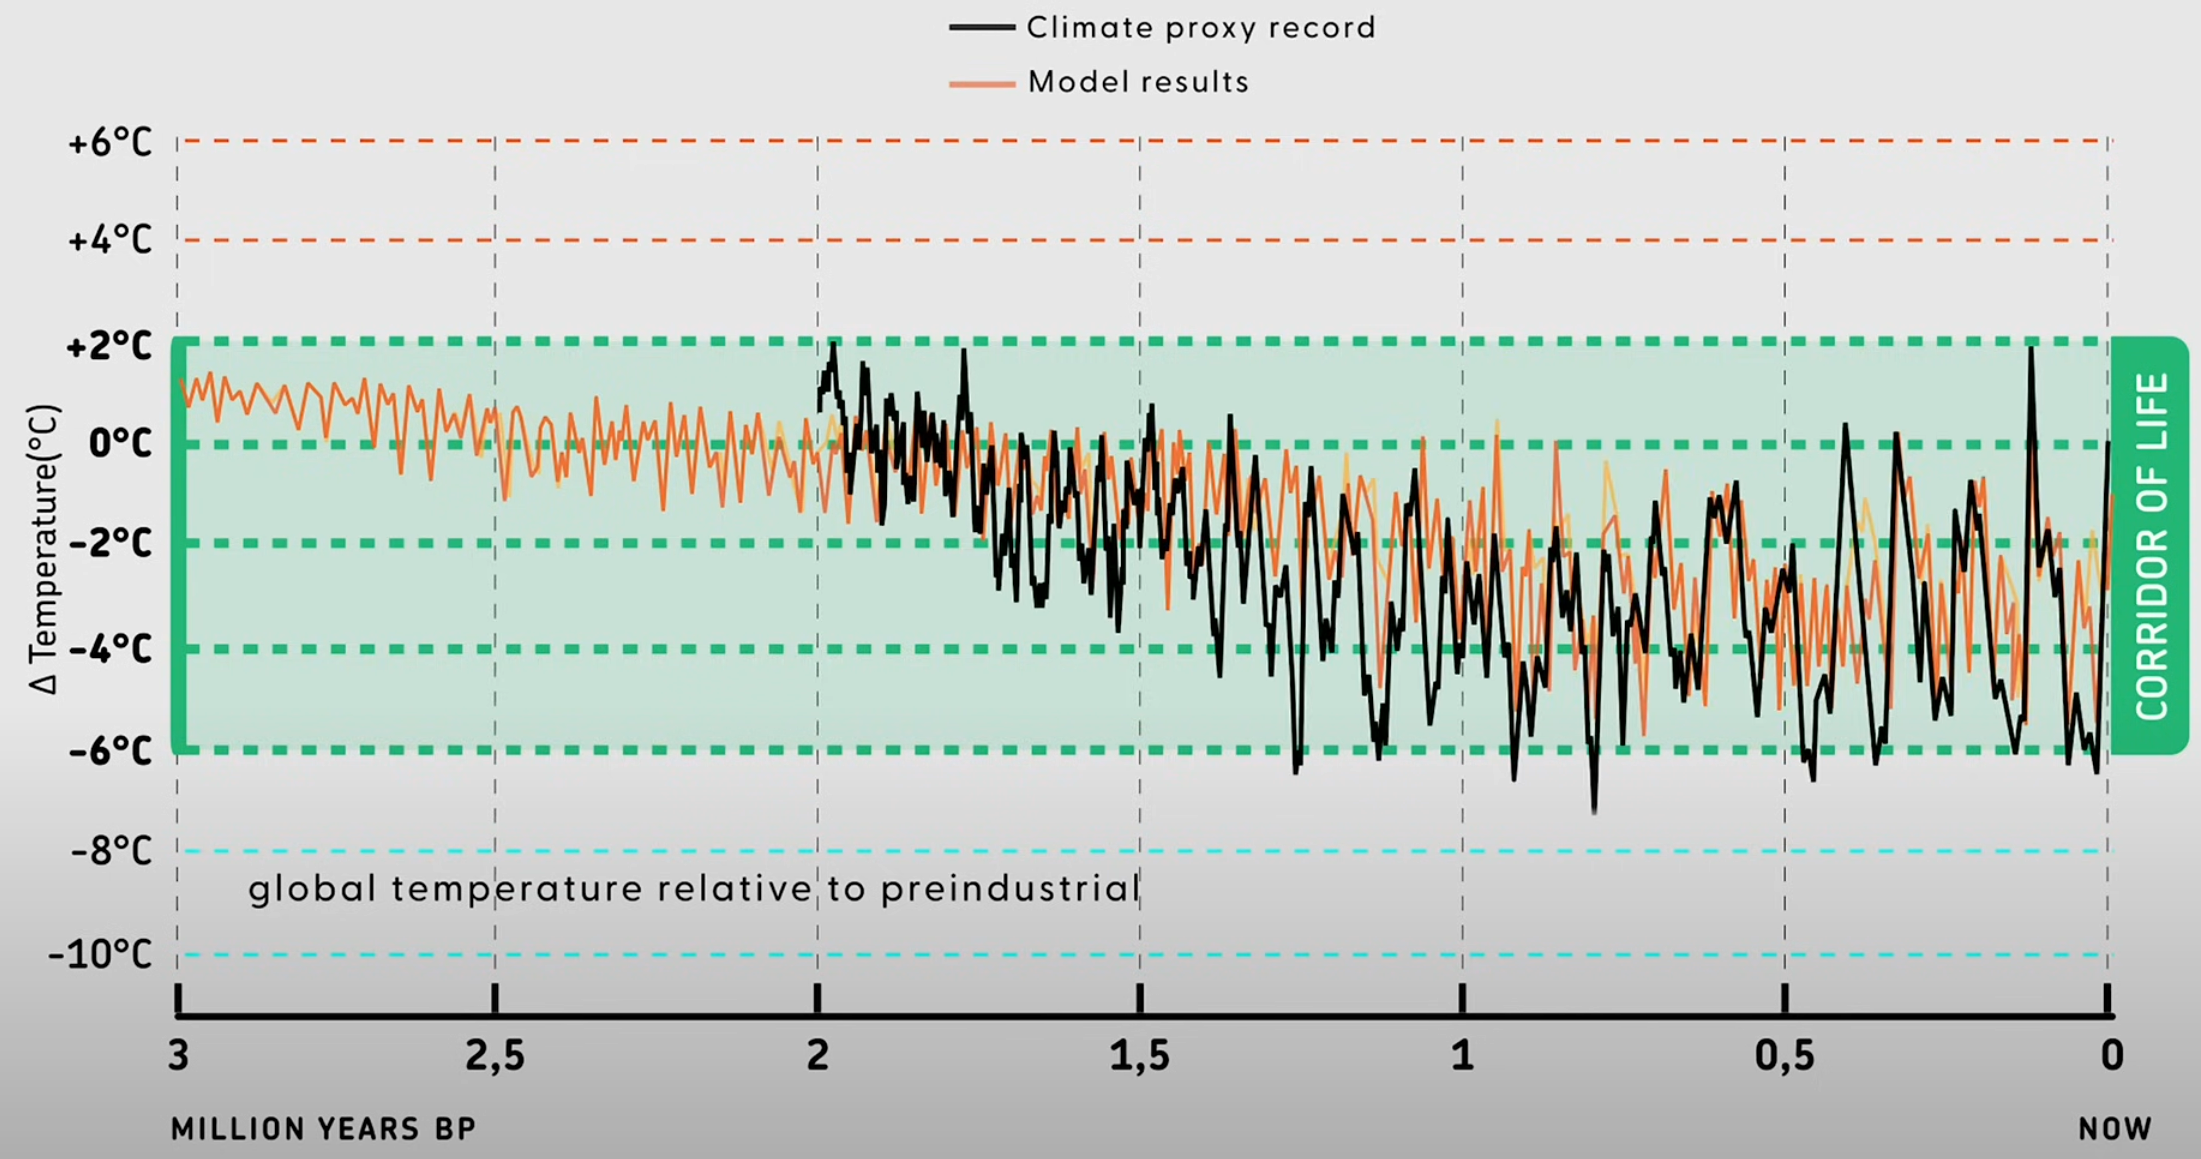
\includegraphics[width=1\linewidth]{images/life_corridor.png}
%     \caption{Enter Caption}
%     \label{fig:intro_life_corridor}
% \end{figure}

%\begin{figure}[H]
%    \centering
%    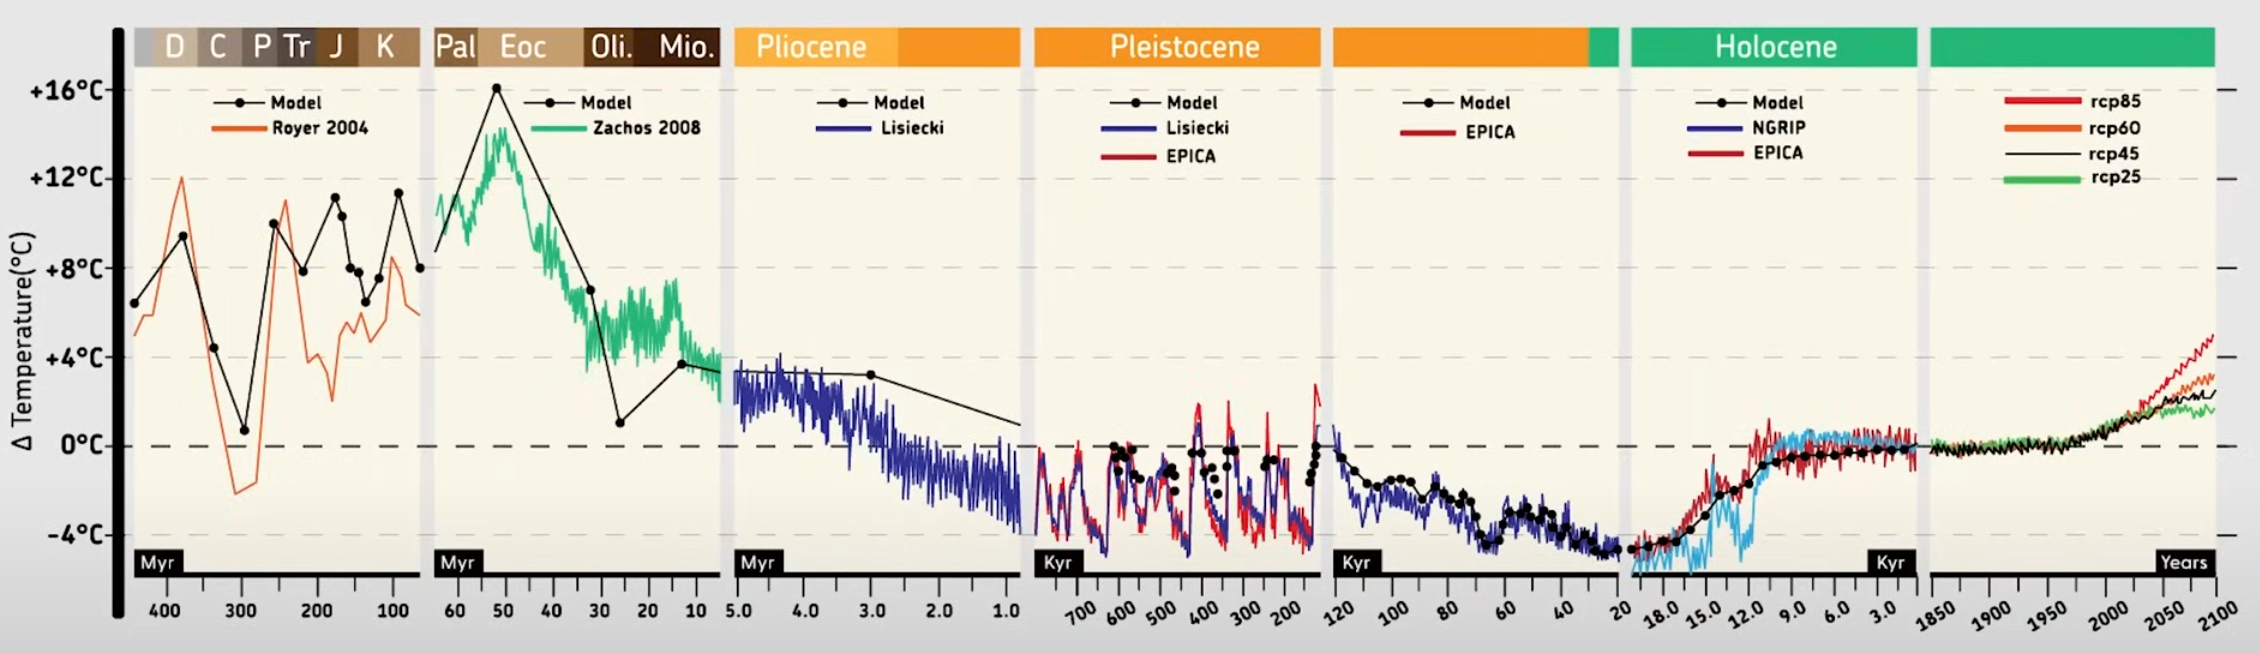
\includegraphics[width=1\linewidth]{images/paleoclimateDT.png}
%    \caption{Enter Caption}
%    \label{fig:placeholder}
%\end{figure}

%\begin{figure}
%    \centering
%    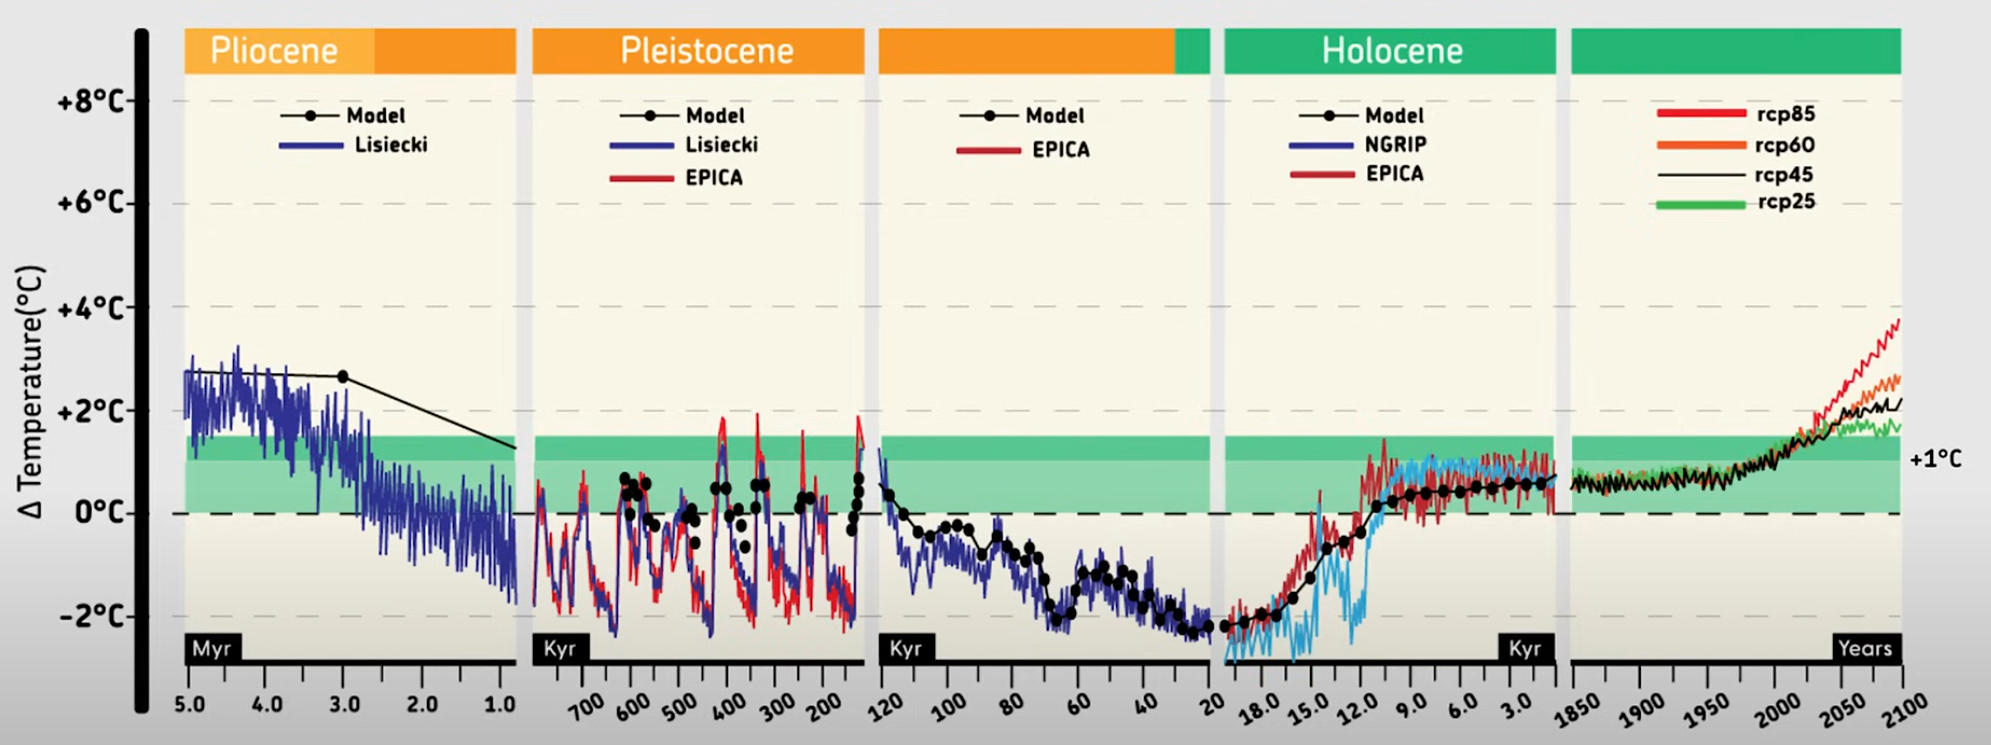
\includegraphics[width=1\linewidth]{images/paleoclimateDT_life_corridor.png}
%    \caption{Enter Caption}
%    \label{fig:placeholder}
%\end{figure}

% \begin{figure}
%     \centering
%     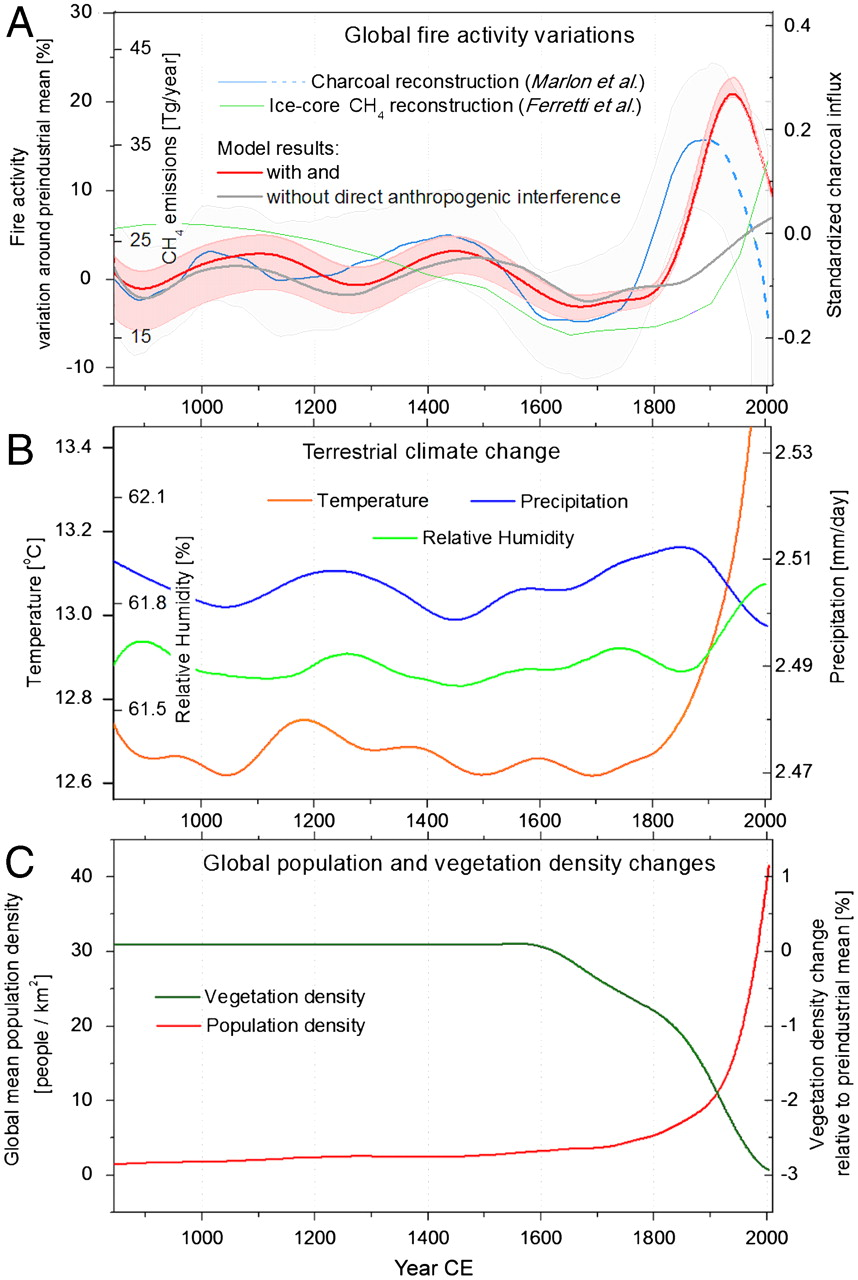
\includegraphics[width=0.7\linewidth]{images/paleo_globa_fire_activityVSpopulation_temperature.png}
%     \caption{Global fire activity, climate, vegetation, and population. (A) Modeled global fire activity variations (SI Text) with (red line) and without (gray line) direct anthropogenic influence (ignition and suppression): Red-shaded area represents uncertainty in the anthropogenic effect assumptions (SI Text); ice-core methane fire emissions reconstruction (green line) (17) and charcoal-based global fires reconstruction (blue line) with gray-shaded confidence interval (12) and blue dashed line indicating increased uncertainty in the late 20th century reconstructions. (B) GISS GCM annual means of the terrestrial area surface temperature (orange line), precipitation (blue line), and relative humidity (green line). (C) Global mean population (red line) and vegetation (green line) densities (11).}
%     \label{fig:intro_fire_activity_population}
% \end{figure}
In Earth System science, the \emph{Anthropocene} is an era where human activities act as a planetary force influencing geological, climate, and biospherical systems. This period is marked by extreme or
frequent fires that signal \emph{systemic stress} and possible \emph{critical transitions} in ecosystems and societies
\cite{bowman2020fires,scheffer2009early}. Therefore, socio-ecological
systems must adapt rapidly to conditions that favour intense fire seasons; we
need forecasts and alerts with \emph{high spatial--temporal detail},
operating \emph{day/night} (visible/thermal infrared) and in \emph{any weather}
(microwave/SAR), across urban and rural regions. To this end, it is necessary
to \emph{develop a satellite constellation for fire-meteorology monitoring
with high spatial and temporal resolution}, which---when coupled with other
models and forecasting systems---can provide:
\begin{enumerate}\setlength{\itemsep}{0pt}\setlength{\parskip}{0pt}\setlength{\parsep}{0pt}
\item \textbf{Diagnosis of fire-resilience states \inlineReq{R1}}\footnote{[\rightarrow R\#] refers to the requirement number \# being created at this point. Full description of the requirment is found in the end of each chapter, i.e \S \ref{sec:requirements_level1}.The requirements framework adopted in this work is detailed in Appendix~\ref{app:se_approach} and \S\ref{sec:requirements_level1}.}
\item \textbf{Anticipation of ignitions \inlineReq{R2}}
\item \textbf{Near--real-time identification of hotspots \inlineReq{R3}}
\item \textbf{Near--real-time monitoring of fire-front evolution \inlineReq{R4}}
\item \textbf{All weather, cloud/smoke-penetrating, day/night capability \inlineReq{R5}}
\end{enumerate}


Thus, the constellation gives responders the ability to \emph{suppress
	hotspots as early as possible} and to focus resources where most needed,
given predicted fire evolution and risk---reducing losses of
\emph{biodiversity} and \emph{CO\textsubscript{2} sinks}, which are crucial for
limiting warming and moderating future fire seasons \cite{kelly2020fire}.

As a first step, we propose a \emph{regional-coverage satellite
	constellation design demonstration} for the \emph{Iberian Peninsula
	(continental Portugal)}\inlineReq{R6}. This is a Mediterranean hotspot where wildfire danger
and impacts are among Europe's highest, reflecting strong couplings
between urban systems and fire-prone ecosystems that affect
environmental quality and public well-being \cite{sanmiguel2018fires,costa2020wildfire,turco2019drivers}. From
this \emph{seed constellation}, expansion to other regions is
envisaged.

\section{Motivation \& Problem Statement}\label{sec:motivation}

The motivation for this work can be understood in five points which will be detailed in the following sub-chapters and concluded with the problem statement of this work, they are: first, the climate crisis, which is increasing fire danger; second, the fact that Portugal is a region where fire lines are zoned; third, a need of strengthen of the capabilities wildfire combat in Portugal; fourth, the Portuguese services uses satellite imagery with long revisit period for fire prediction, this high latency image input  directs to the final motivation point,  leading to low fidelity fire spread models predictions and a higher risk of ineffective firefighting. The low fidelity is due the fact the weather is dynamic and the changes between measurments are not certain, the uncertain grows with time, increasing the impression of the models, therefor high cadence satellite imaginary is needed to avoid low fidelity.  These are the key points that motivate the development of a high-temporal and spatial satellite constellation to improve fire prediction and management in Portugal. 

\subsection{Climate crisis with increased fire danger} 

Anthropogenic warming has lengthened fire-weather seasons globally from ${\sim}60$\,days\,yr$^{-1}$ (2025 baseline) toward ${\sim}70$\,days by mid-century and ${\sim}78$\,days by 2100, while the frequency of extreme fire-weather days ($\mathrm{FWI}_{95\mathrm{d}}$) has risen in step \cite{jones_global_2022,abatzoglou_global_2019}. The signal is strongest in the Mediterranean, where fire-season length is projected to grow from ${\sim}90$ to ${\sim}150$\,days\,yr$^{-1}$ and extreme days from ${\sim}30$ to ${\sim}75$\,days\,yr$^{-1}$ over the same horizon. Although \emph{global} burned area has declined since 2001---driven primarily by African savanna land-use change---regional burned area in Mediterranean and boreal forest biomes has increased, with Mediterranean projections of $+40$--$187\%$ under $1.5$--$3\,^{\circ}$C warming scenarios \cite{jones_global_2022,andela_humandriven_2017,turco_exacerbated_2018}.

Senande-Rivera et al.\ classified fire-prone regions worldwide into four K\"oppen--Geiger-based fire-climate classes, each stratified by recurrence: \emph{recurrent} ($>7$ fire-prone years per decade), \emph{occasional} ($3$--$7$), and \emph{infrequent} ($<3$) \cite{senande-rivera_spatial_2022}. Their projections (2070--2099) shown that some presently infrequent zones shift to occasional and occasional zones tend to become recurrent, enlarging the global fire-prone area (Fig.~\ref{fig:fire_prone_global_now_future}). This classification is adopted in Section~\ref{sec:generalized_study_domain} to define the constellation's global study domain $\mathcal{D}_{\text{Global}}$ fire-prone target mask.

\begin{figure}[H]
    \centering
    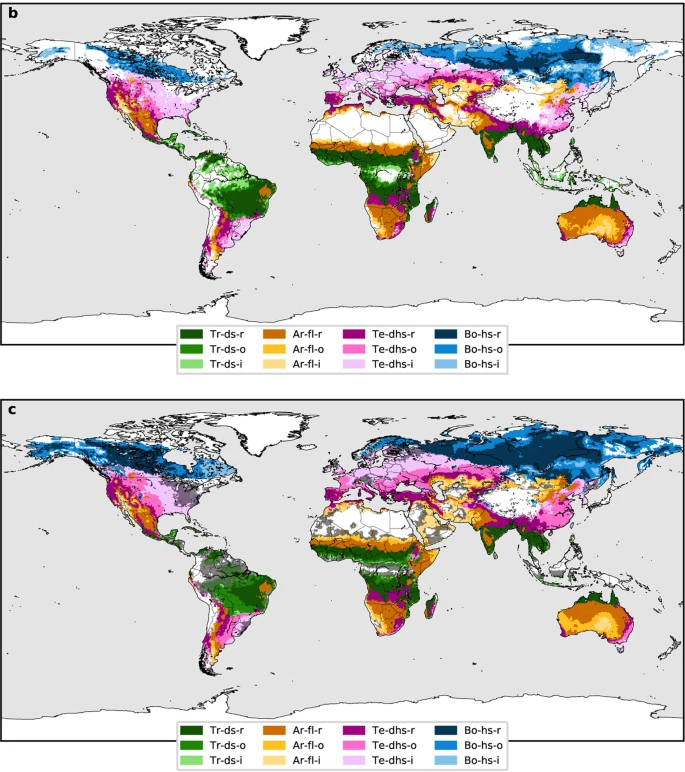
\includegraphics[width=0.9\linewidth]{images/fire_prone_global_now_future.png}
    \caption{\footnotesize{Present and projected global fire-prone climatic regions. (b)~Present fire-climate regions (1996--2016). (c)~Projected fire-climate regions (2070--2099) under CMIP5 GCMs; shaded grey indicates $<$75\% model agreement. Four fire-climate classes---Tropical-Dry Season (Tr-ds), Arid-Fuel Limited (Ar-fl), Temperate-Dry Hot Season (Te-dhs), Boreal-Hot Season (Bo-hs)---are each subdivided by fire-prone year recurrence per decade: recurrent~(r,\,$>$7), occasional~(o,\,3--7), infrequent~(i,\,$<$3). Adapted from Senande-Rivera et al.\ \cite{senande-rivera_spatial_2022}.}}
    \label{fig:fire_prone_global_now_future}
\end{figure}


% \subsection{Recent increase of fire danger (global/European signal).}

% Assessments show robust increases in \emph{fire weather}, longer
% seasons, and projected growth in burned area under continued
% warming---signals that are particularly strong across Iberia and the
% broader Mediterranean \cite{ipcc2023syr,jolly2015climate}.

\subsection{Portugal: recurrent, severe wildfires.} 


Continental Portugal exemplifies these challenges, with repeated extreme seasons;
\emph{2017} stands out as catastrophic in scale and impacts (area
burned, 116 fatalities and hundreds wounded), motivating improved observation and response
capability \cite{sanmiguel2018fires,turco2019drivers,cti2017pedrogao}. A prominent example with 66 fatalities is the
\textbf{17 June 2017 Pedrógão Grande} event: under \emph{extreme	pyrometeorology}, the convective column collapsed, producing a \emph{downburst} that drove the fire front at \emph{\textasciitilde15 km h$^{-1}$ for \textasciitilde10min}---overwhelming decision windows, for reference, human average running speed is \textasciitilde10 km h$^{-1}$---at a time when \emph{near--real-time orbital nowcasting} was not integrated into operations \cite{cti2017pedrogao}.

In 2025, Portugal’s burned area approached \(\sim\)280{,}000~ha (\(\approx\)3\% of national territory), rivaling 2017, with major fires affecting Castelo Branco (incl. the Fundão area) \cite{portugal_area_2025, effisPRTstats, reuters2025eu,}. Evidence from the Mediterranean shows that land abandonment and the resulting increases in fuel load/connectivity elevate fire hazard and the likelihood of large events; abandoned farmland transitioning to shrubland is particularly at risk \cite{schworer2024medfire,kirkland2024med}. Species composition also modulates hazard: eucalypts display high flammability traits that can promote intense fire behaviour, though in Portugal the expansion of eucalypt plantations alone does not explain interannual burned area once weather and other drivers are accounted for \cite{younes2024eucflamm,fernandes2019eucalypt}. These dynamics strengthen the case for high-cadence Earth observation to support early detection, nowcasting, and operational decision-making during transitions toward more resilient urban–rural–forest socio-ecosystems.

\begin{figure}[H]
    \centering
    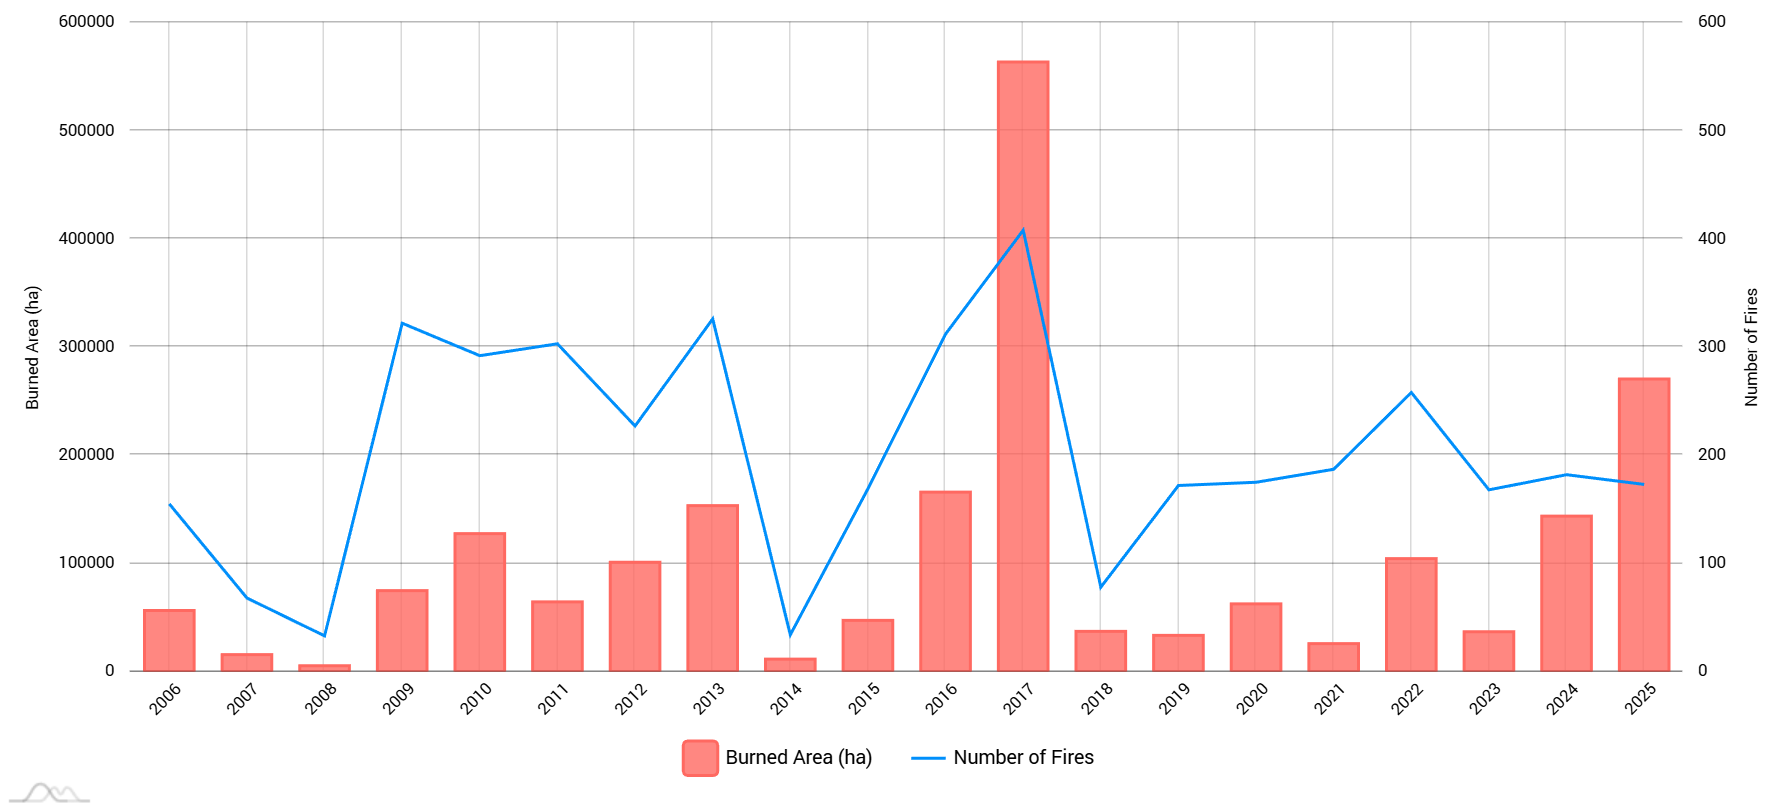
\includegraphics[width=1\linewidth]{images/burned_area_estimates-by-country_PRT_2006_2024.png}
    \caption{\footnotesize{EFFIS annual burned area statistic temporal series for Portugal. Two charts of temporal series between 2006 and Setember-2025 showing burned area and number of Fires.\protect\footnotemark}}
    \label{fig:burned_area_estimative_pt}
\end{figure}
\footnotetext{Reproduced from Abatzoglou, J.~T., Williams, A.~P., \& Barbero, R. (2019), \textit{Geophys. Res. Lett.} 46, 326–336, doi:10.1029/2018GL080959. 
\copyright~2019 American Geophysical Union.\cite{effisPRTstats}}


\begin{figure}[H]
    \centering
    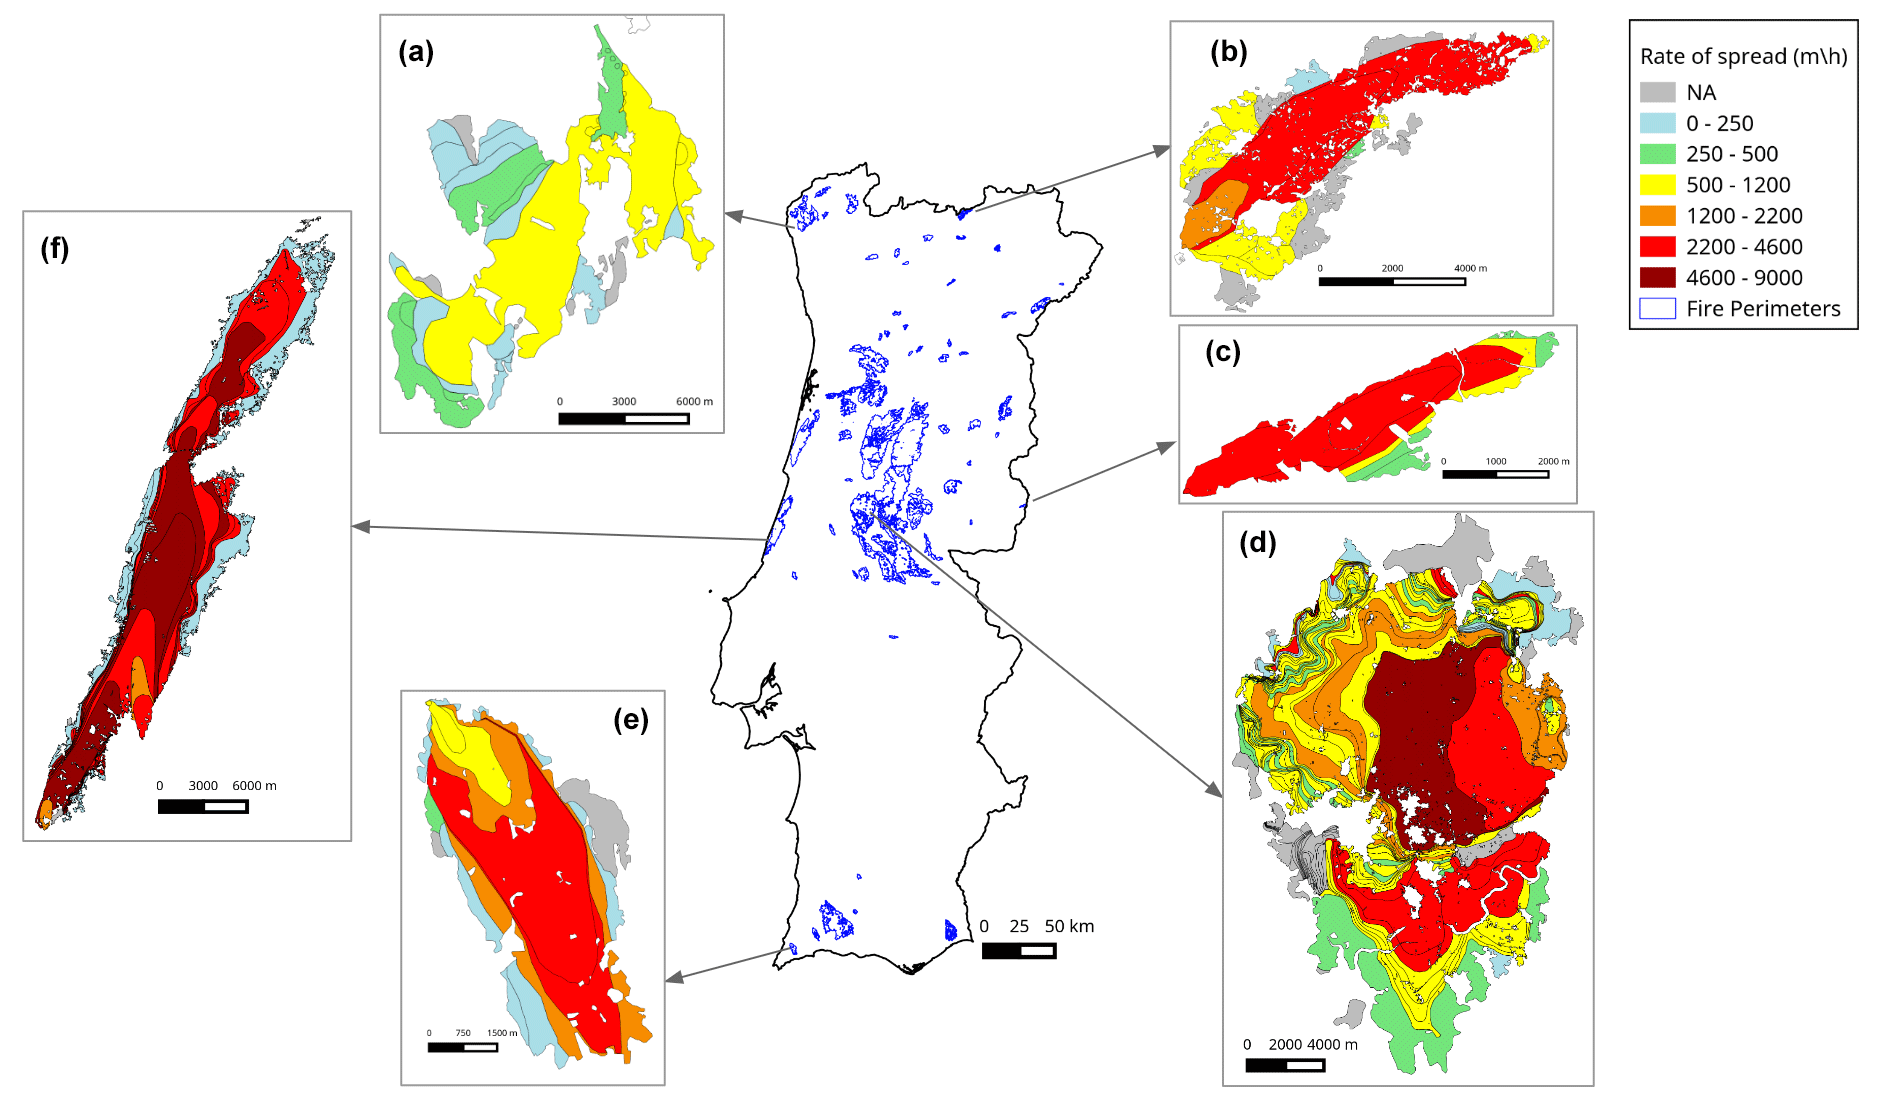
\includegraphics[width=1\linewidth]{images/Overall_spatial_distribution_of_wildfire_perimeters_in_Pt.png}
    \caption{\footnotesize{The distribution of wildfires in Portugal was analyzed using the Pt-FireSprd database project between 2016-2020.\cite{benali2023ptfiresprd} The perimeters show an analysis of the fire rate of spread (ROS) for six wildfires: (a) Paredes de Coura (2016), (b) Chaves (2020), (c) Idanha-a-Nova (2020), (d) Pedrógo Grande (2017), (e) Aljezur (2020), and (f) Alcobaça (2017).}}
    \label{fig:distribution_wildfire_rate_of_spread}
\end{figure}


\begin{figure}[H]
    \centering
    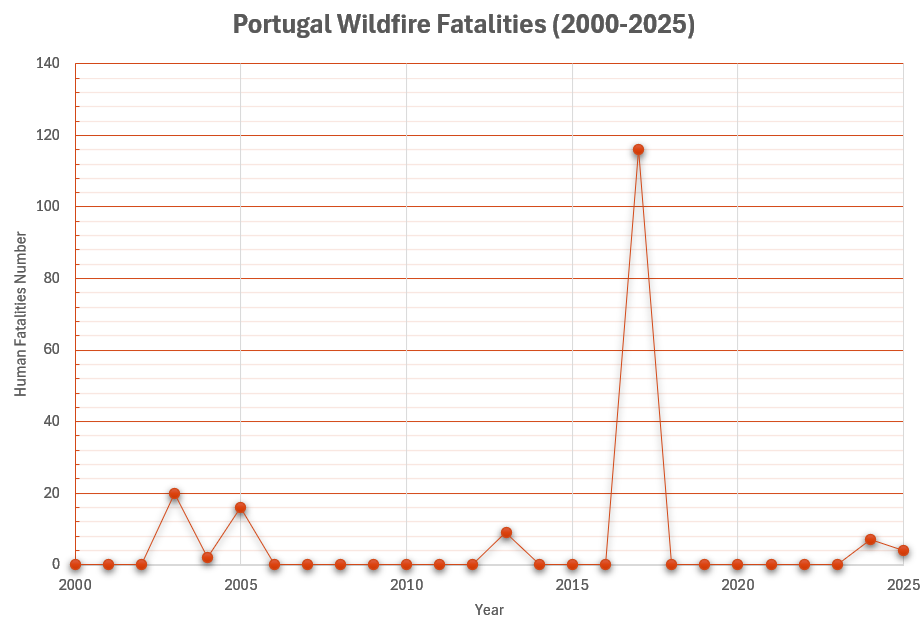
\includegraphics[width=0.75\linewidth]{images/wildfire_fatalities_pt.png}
    \caption{\footnotesize{Annual wildfire fatalities in Portugal (2000–2025). Key values from CTI reports for 2017 \cite{CTI2017_June,CTI2018_October}, MAI (2013) \cite{MAI2013_Accidents}, Viegas (2009) and Rodrigues et al. (2022) for 2003/2005 \cite{Viegas2009_CercadosParteII,Rodrigues2022_RuralFiresLosses}, and AGIF for 2023 \cite{AGIF2024_SGIFR2023}; 2024–2025 are provisional \cite{Reuters2024_PortugalWildfires,ECHO2025_PortugalFiresFlash}.}}
    \label{fig:pt_wildfire_fatalities}
\end{figure}
\footnotetext{Reproduced from Abatzoglou, J.~T., Williams, A.~P., \& Barbero, R. (2019), \textit{Geophys. Res. Lett.} 46, 326–336, doi:10.1029/2018GL080959. 
\copyright~2019 American Geophysical Union.\cite{effisPRTstats}}


% \vspace{1.5em}
\subsection{Need for strengthening the current Portuguese Earth Observation Capabilities for wildfire managemen}

Spaceborne assets are invaluable but split between \emph{coarse, frequent geostationary} views and
\emph{finer, infrequent polar} passes; performance can degrade under smoke/cloud, and \emph{small/fast ignitions are often detected late}, limiting time-to-first-intervention and model fidelity
\cite{wooster2021review}. Portugal has an integrated wildfire management system 
involving multiple agencies under the Agência para a Gestão Integrada de Fogos Rurais 
(Agency for Integrated Rural Fire Management, AGIF). 
AGIF sets the national policies and strategies for wildfire prevention and control.

Besides ground sensors, AGIS’s fire combat system uses typical satellite imagery 
like \emph{Sentinel-2}, which has a \emph{nominal 5-day revisit} to the same Earth’s region of 
interest, in other words, \emph{5 days of temporal resolution}\cite{esa_s2_facts}. 
This doesn’t match the hourly-scale dynamics of ignition and early spread.

% \vspace{1.5em}
\subsection{Low-fidelity Fire Weather Prediction}

Within the \emph{ImFire} project at the \emph{Association for the Development of Industrial Aerodynamics} (Associação para o Desenvolvimento da Aerodinâmica Industrial, ADAI), the workflow runs fire-spread models to forecast behavior and likely propagation corridors\cite{pereira_metaheuristic_2024}. However, in practice, these models rarely directly use satellite images for ignition location or active fireline geolocation because available EO streams usually lack the necessary temporal cadence and/or spatial detail for hour-scale operations (e.g., Sentinel-2’s roughly 5-day revisit). Therefore, ImFire mainly depends on meteorology, fuels, topography, and operational reports from ground sensors or aircraft, while satellite data are more often used for situational awareness or post-event mapping than for real-time model input.

% \vspace{1.5em}
\subsection{New Faster Constellation Requirements}

The performance of an alert system earth observation satellite constellation is mostly defined by two parameters: the time interval between consecutive passes of one spacecraft over the same Earth spot, defined as \textbf{temporal resolution} $\Delta t$ or $t_{\text{revisit}}$, and the space platforms imaging capability to resolve the ground scene from the spacecraft's perspective, defined as \textbf{spatial resolution $\Delta s$ or Ground Sample Distance (GSD)}. 

A dedicated satellite constellation could offer the requisite high temporal and spatial resolution, exceeding existing capabilities in fire weather forecasting. The ImFire team is collaborating with this thesis and has proposed a set of requirements to better suit their models. They have indicated that a \textit{satellite constellation} with a \textbf{temporal resolution $\mathbf{{t_{revisit} \approx 30}}$} minutes and a \textbf{spatial resolution\textbf{ }$\mathbf{{GSD \approx 6 \text{ \textbf{m/pixel}}}}$  }would \textit{significantly improve the accuracy of fire model predictions}\inlineReq{R7}, \inlineReq{R8},
\cite{ipcc2023syr,pereira2024fire,benali2023ptfiresprd}.

Figure \ref{fig:gap_satellite_constellations_spatial_temporal_plot} shows the gap in the know state of the art of low Earth orbit satellite constellations for fire detection. The target for this thesis, the Constellation Satellite $\mathcal{C}_{\text{sat}}$ design, is plotted at a temporal resolution of approximately 30 minutes and a spatial resolution of around 6 meters per pixel, which lies beyond the existing performance frontier and motivates the orbital architecture developed in this work.

\begin{figure}[H]
    \centering
    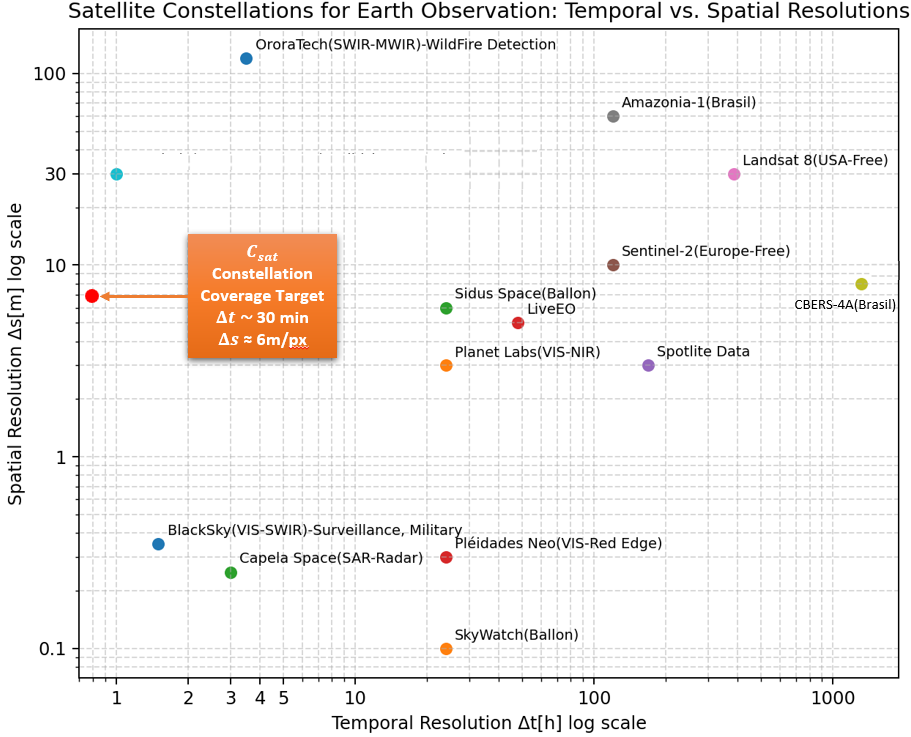
\includegraphics[width=1\linewidth]{images/satellite_constellations_spatial_temporal_plot.png}
    \caption{\footnotesize{Spatial resolution (GSD) vs.\ temporal resolution (revisit time) for known LEO satellites and constellations capable of fire detection. Mission target $\mathcal{C}_{\text{sat}}$.}}
    \label{fig:gap_satellite_constellations_spatial_temporal_plot}
\end{figure}


\begin{tcolorbox}[colback=white, colframe=black, title=\textbf{Problem Statement}]
\emph{Wildfire risk in Mediterranean Europe}---including Portugal---has intensified under the Great Acceleration \cite{steffen2015trajectory}, with projections indicating significant \emph{rises in fire weather}, \emph{longer seasons}, and \emph{larger burned area across Iberia} \cite{ipcc2023syr,jolly2015climate, pereira2024fire, benali2023ptfiresprd}. Catastrophic episodes such as \emph{Pedrógão Grande (2017)} show how, under extreme \emph{pyrometeorology}, \emph{fire fronts can accelerate and overwhelm decision windows}---and that \emph{near--real-time orbital detection/nowcasting was not integrated into operations} at the time \cite{cti2017pedrogao}. Current satellite services face a \emph{resolution--revisit--latency gap}: \emph{coarse/frequent GEO} plus \emph{finer/infrequent LEO} often \emph{miss or delay} small, fast-moving ignitions and \emph{degrade under smoke/cloud}, constraining timely intervention and model fidelity \cite{wooster2021review,esa_s2_facts}. Moreover, \emph{Portuguese fire-prediction workflows} depend on Sentinel 2 inputs whose \emph{temporal cadence} of 5 days and spatial resolution for the fire prediction application of $30 \text{m/px}$ is insufficient for hour-scale dynamics; improving forecast capabilities requires \emph{high-frequency, high-resolution} EO data \cite{pereira_metaheuristic_2024}. 

\vspace{1em}
\textbf{Scientific problem:} a mismatch between \emph{the temporal/spatial scale of fire dynamics} and the \emph{capability of existing orbital observation systems for fire management}---which raises the central research question: \emph{what satellite constellation design can close this spatiotemporal gap, improving fire-weather and fire-spread prediction for Portugal?}
\end{tcolorbox}


\section{Aim and Scope}\label{sec:aim-and-scope}

\begin{tcolorbox}[colback=white, colframe=black, title=\textbf{Aim}\label{aim}]
To design an \emph{orbital architecture} for a small-satellite constellation that enables \emph{minute-scale revisit ($\approx$30 min), meter-scale detail (\textasciitilde6 m GSD), day/night and all-weather	visibility, and low end-to-end latency} over \emph{continental Portugal}, sufficient to \emph{improve fire-weather and fire-spread model inputs} and \emph{support tactical decision-making}, and to analyze the coverage reach of the proposed constellation over regional and global fire-prone regions.
\end{tcolorbox}

\emph{Scope}\label{scope}

What this work will cover and not cover?
\vspace{1.5em}

\emph{In scope:}

\begin{itemize}
	\item
	      \textbf{Orbital architecture design:} High-fidelity mission simulation using  GMAT and Orekit to analyze Kepler parameters, altitude/inclination selection, comparison between Sun Synchronous Orbit and Repeating Ground Track Orbit, non-resonant orbits, plane count and spacing, single vs. multi-layer constellations, and phase management.
	\item
	      \textbf{Coverage \& performance analysis:} access time, mean/worst-case revisit, probability of access within operational windows, geometry needed to achieve target GSD over Portugal; seasonal/diurnal effects, groundtrack coverage.
	\item
	      \textbf{Sensitivity studies:} number of satellites, altitude, RAAN
	      spacing, temporal coverage maps; trade-offs among revisit, GSD, and
	      latency.
	\item
	      \textbf{Implications for sensing (high level only, optional time dependent):} derive
	      \emph{top-level sensor family requirements} implied by the chosen
	      architecture (e.g., optical/thermal/microwave, day/night/all-weather),
	      \emph{without} detailed payload design.
        \item
          \textbf{Communications \& latency budgets(optional, time dependent):}
          inter-satellite links vs. direct-to-ground, ground-station network
          options, onboard vs. ground processing assumptions,
          \emph{detection-to-decision} timing analysis.
\end{itemize}

\emph{Out of scope:}

\begin{itemize}
	\item
	      \textbf{Detailed payload engineering:} detector/optics/radiometry
	      design, SNR/NE$\Delta$T budgeting, thermal/power/mechanical design,
	      calibration/validation plans.
	\item
	      \textbf{Algorithm development:} new fire-detection or spread-model
	      algorithms beyond using published performance assumptions for
	      cadence/latency needs.
	\item
	      \textbf{Operational coupling at a high level:} mapping cadence/latency
	      to \emph{model-update frequency} and
	      \emph{time-to-first-intervention}; conceptual interfaces with
	      existing Portuguese workflows (e.g., AGIF/ImFire).
	\item
	      \textbf{Programmatics/economics:} cost models, procurement,
	      regulatory/licensing and spectrum coordination.
	\item
	      \textbf{Full operational integration \& field deployment:} end-to-end
	      real-world trials or system acquisition; global designs beyond
	      Portugal (except brief generalization notes).
\end{itemize}


\section{Significance of the Study}\label{sec:significance}

This work addresses a documented gap in the fire-detection state of the art: no existing or planned satellite constellation combines sub-hour revisit with metre-scale ground resolution over fire-prone regions.
The orbital architecture and design methodology developed here provide a transferable framework for closing that gap---first for Portugal, then for any fire-prone latitude worldwide.

\section{Structure of the Thesis}\label{sec:structure}

This thesis follows a NASA/ESA systems-engineering life-cycle scoped to Pre-Phase~A and Phase~A (the full methodological framework is detailed in Appendix~\ref{app:se_approach}). The narrative moves from evidence $\rightarrow$ needs $\rightarrow$ concepts $\rightarrow$ simulation trades $\rightarrow$ baseline solution, organised in three parts.


\begin{figure}[H]
	\centering
	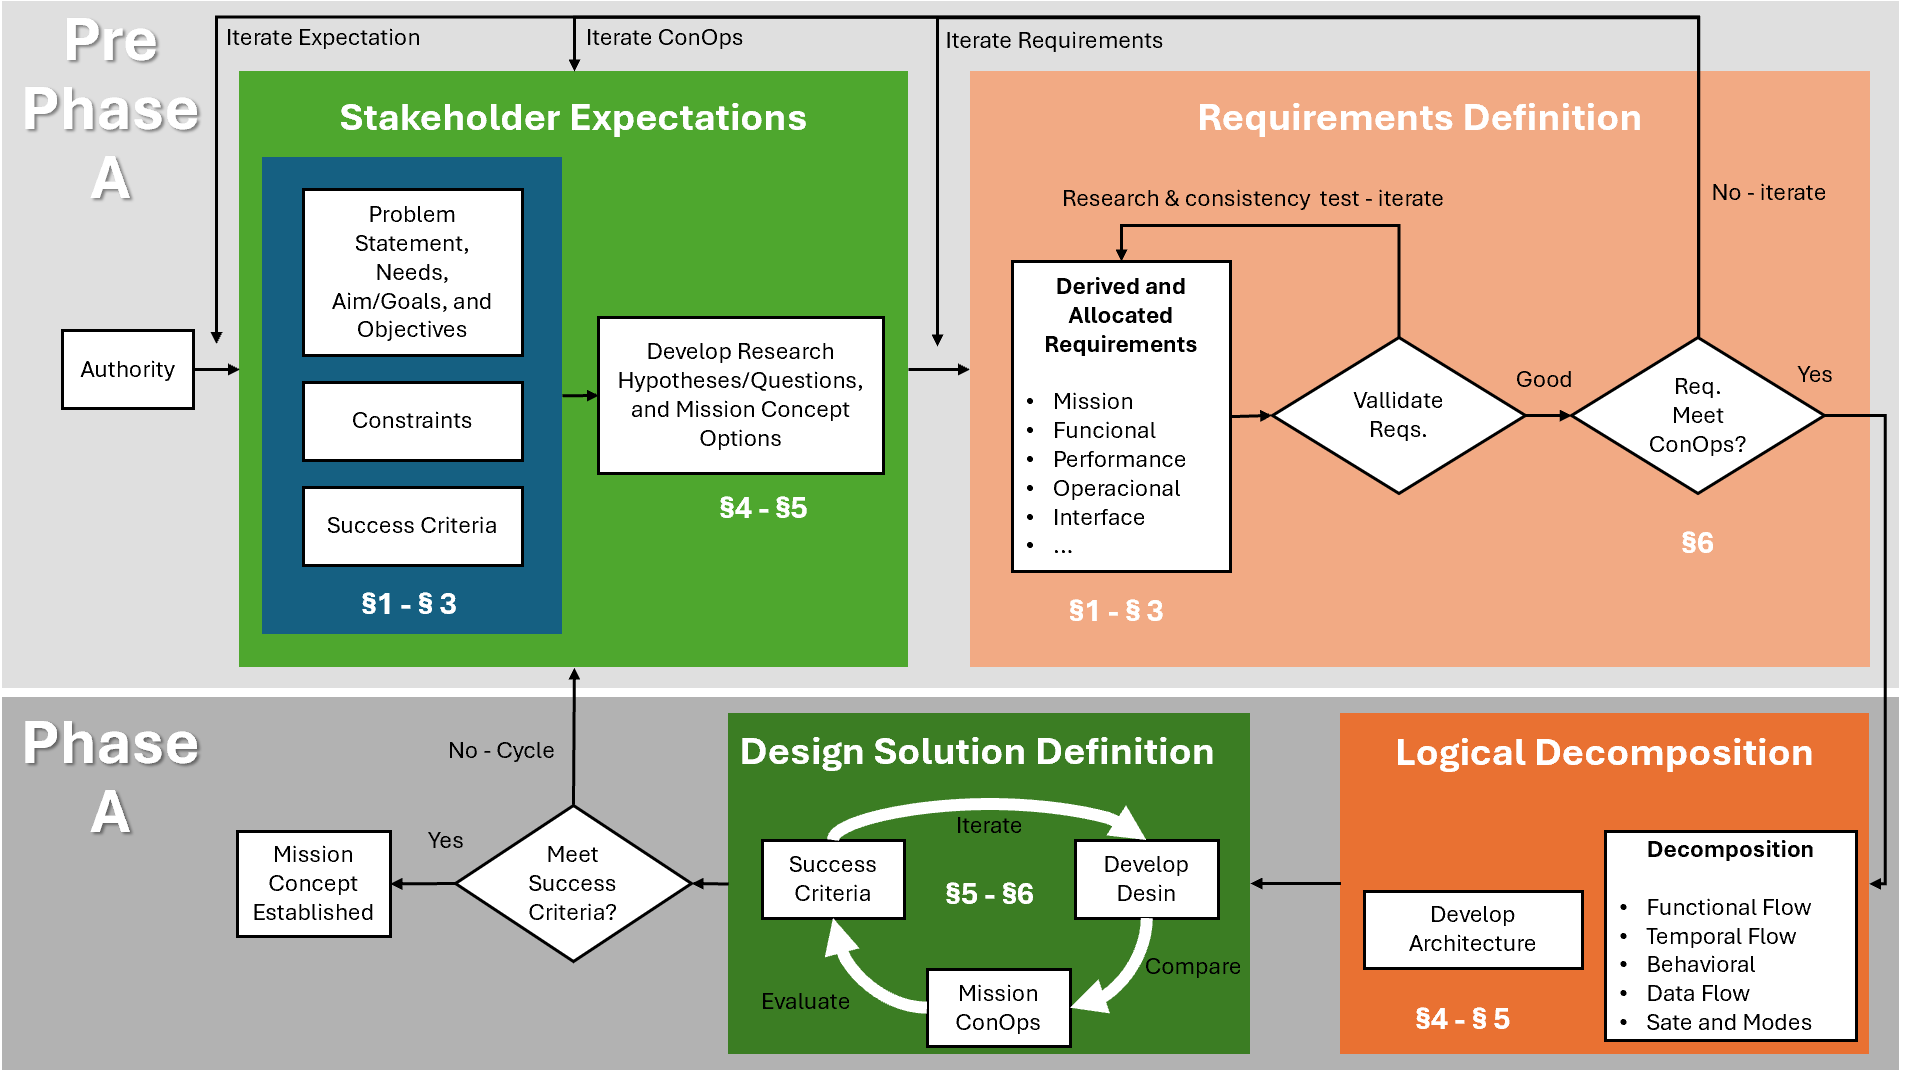
\includegraphics[width=1\textwidth]{images/c1.4.2_Interrelationships_SE_PrePhase_A_Phase_A.png}
	\caption[Connections between Pre-Phase A and Phase A system design processes. The chapters where these processes are discussed are highlighted with the symbol \S. Adapted from]{Relation between Pre-Phase A and Phase A system design processes. The chapters where these processes are discussed are highlighted with the symbol \S. Note the Stakeholder Expectation and Requirements Definitions overlap in chapter \S1 - \S5. Adapted from \parencite{SEHandbook}.}
	\label{fig:nasa-lifecycle_prephaseA-phaseA}
\end{figure}


PART I (Chs. 1--3) establishes the problem context, study domains, and physical foundations (Pre-Phase A). 
Chapter 1 states the context, motivation, aim, and scope, framing the spatiotemporal observation gap that motivates the thesis. 
Chapter 2 defines the Core Study Domain ($\mathcal{D}_{core}$, mainland Portugal) and Global Study Domain ($\mathcal{D}_{global}$, Earth's fire-prone regions), establishing spatial, temporal, and reference-data boundaries. 
Chapter 3 develops the radiometric and geometric physics of fire remote sensing from orbit, deriving the observation constraints that drive sensor and constellation requirements. 

PART II (Chs. 4--5) starts Phase A with theory and architecture trade-offs. 
Chapter 4 presents the constellation-design fundamentals: observation formalism, orbital mechanics, visibility geometry, and Repeating Ground Track Orbit theory, including a quantitative comparison with Sun-Synchronous Orbits that justifies the RGTO selection. 
Chapter 5 explores the Walker RGTO design space, selects seed orbital parameters, and defines the plane count and satellite phasing to satisfy the revisit requirements over Portugal. 

PART III (Chs. 6--8) presents and interprets outcomes. 
Chapter 6 synthesises the results of the baseline 15-satellite constellation and the two-layer Watcher--Zoom tip-and-cue architecture. 
Chapter 7 discusses feasibility, limitations, and transferability of the results, 
and Chapter 8 concludes by answering the research questions and outlining avenues for future work. 

Six appendices provide supporting derivations and data: the geopotential $J_2$ model (A), the SSO-vs-RGTO benchmark (B), station-keeping and orbit lifetime (C), Walker RGTO element tables (D), the consolidated requirements list R1--R25 (E), and the full systems-engineering methodological framework (F).


\section{Requirement Mission Objectives and Level-1 Summary}\label{sec:requirements_level1}

This subchapter presents the chapter 1 insights as mission requirements, formatted in a systems engineering style. It provides a complete description of mission needs. The table below supports traceability and reference for theory, methodology, simulation constraints, and expected results.

\vspace{\baselineskip}
Requirement table symbolism legend:
\vspace{\baselineskip}

\requirement{R\#}{Requirement Name}{Description of the requirement.}{Req. type}{Subsystem/Parameter/Tag}
\vspace{\baselineskip}


\vspace{\baselineskip}
The complete definition of the mission objectives (R1--R4), environmental constraints (R5), and constellation performance requirements (R6--R8) is provided in Appendix~\ref{sec:app_req_ch1}.
